\documentclass{article}
\usepackage[margin=2cm]{geometry}
\usepackage{graphicx}
\usepackage[pages=some]{background}
\usepackage{titling}
\usepackage{tabularx}
\usepackage{tikz}
\usepackage{forest}
\usepackage{float}
\usepackage{subfigure}

\forestset{
  my box/.style={
    draw,
    rectangle,
    rounded corners,
    fill=gray!20,
    inner sep=6pt,
    minimum width=3cm % Adjust the width as needed
  }
}


\geometry{a4paper}

\backgroundsetup{
    scale=1,
    angle=0,
    opacity=1,
    contents={%
        
\includegraphics[width=\paperwidth,height=\paperheight]{institution_logo.jpg}
    }
}

\newcommand{\subtitle}[1]{
    \posttitle{
        \par\end{center}
        \begin{center}\large#1\end{center}
        \vskip0.5em}
}

\title{ME-463}
\author{Md. Hasibul Islam}
\subtitle{IC ENGINES}

\begin{document}
\begin{titlepage}
    \centering
    
    {\Huge\bfseries\maketitle}
    \textbf{Zahurul Haque Sir} \\
    \vspace{2cm}
    
\includegraphics[width=8cm]{institution_logo.jpg}
    \vfill
    \vspace*{2cm}
\end{titlepage}

\tableofcontents
\pagebreak
\section{Lecture 01: Introduction} 
\hfill Date: 04/06/2023

\section{Lecture 02: ENGINE FUELS} 
\hfill Date: 06/06/2023
\begin{itemize}
  \item In future → Diesel + 5-10\% bio-diesel
  \item In future → Petrol + Ethanol
  \item High H/C ratio indicates high value of energy \& heating
  \item Gasoline : 31,850 kJ/L 
  \item Average Human power in 0.2 hp, but an 1500 cc car has a power of 60 kW
  \item Octane number → Petrol Engines 
  \item Cetane number → Diesel Engines 
  \item High compression ratio → more knocking 
\end{itemize}

\subsubsection*{Octane Number}
The octane number is a rating used to measure the performance of gasoline (petrol) in spark-ignition engines. It indicates a fuel's resistance to knocking or detonation, which is the spontaneous combustion of the fuel-air mixture in the engine cylinder, causing a knocking sound. Knocking can lead to engine damage and reduced efficiency. The higher the octane number, the more resistant the fuel is to knocking.\\
Typically, two common octane rating methods are used: Research Octane Number (RON) and Motor Octane Number (MON). RON measures a fuel's performance under mild operating conditions, while MON evaluates it under more severe conditions. The octane number displayed at gas stations usually refers to the average of RON and MON, known as the Anti-Knock Index (AKI) or Pump Octane Number (PON).\\
Higher octane number is preferable. 


\subsubsection*{Cetane Number}
The cetane number is a rating used to measure the ignition quality of diesel fuel. It represents the fuel's ability to ignite quickly and burn efficiently in a compression-ignition (diesel) engine. Similar to the octane number, the cetane number is obtained through laboratory tests. It measures the delay between fuel injection and ignition in a diesel engine. Higher cetane numbers result in shorter ignition delays and more complete combustion.
\begin{itemize}
  \item It indicates the ability of self-ignite of engine.
  \item Higher cetane number may cause firing easily. 
  \item Lower cetane number creates knocking, and even create an explode of 2000°C.
  \item At lower cetane number, fuel will be mixed properly, because of time lagging. 
  \item Neither high cetane number, nor low cetane number is preferable. 
\end{itemize}

\subsubsection*{Why Octane number should be high, but cetane number should be in a specific range?}
While a higher octane number is generally preferable to resist knocking in spark-ignition engines, the ideal cetane number for diesel fuel is not too high or too low. Here's why:
\begin{itemize}
  \item \textbf{Too High Cetane Number}: If the cetane number of diesel fuel is excessively high, it can lead to a phenomenon known as "cetane number related ignition delay." This means the fuel ignites too quickly during the compression stroke, causing a rapid rise in pressure. This can result in increased engine noise, rough combustion, and potentially higher emissions.
  \item \textbf{Too Low Cetane Number}: On the other hand, if the cetane number is too low, the fuel may have a longer ignition delay, causing a delayed start of combustion in the diesel engine. This can lead to difficult cold-starting, rough idling, reduced engine performance, and increased emissions.
\end{itemize}

To achieve optimal performance, diesel fuels are typically formulated to have cetane numbers within a specified range that balances ignition quality, combustion efficiency, and emissions control. The specific range may vary depending on engine design, regional fuel standards, and operating conditions.It's important to note that the cetane number requirements may differ for different diesel engines and applications. For instance, high-performance engines or heavy-duty diesel engines may have different cetane number recommendations compared to standard passenger vehicle diesel engines. By maintaining an appropriate cetane number range for diesel fuel, it ensures proper ignition characteristics, smooth combustion, good cold-starting performance, improved fuel efficiency, and reduced emissions in diesel engines.

\begin{figure}
  \centering
  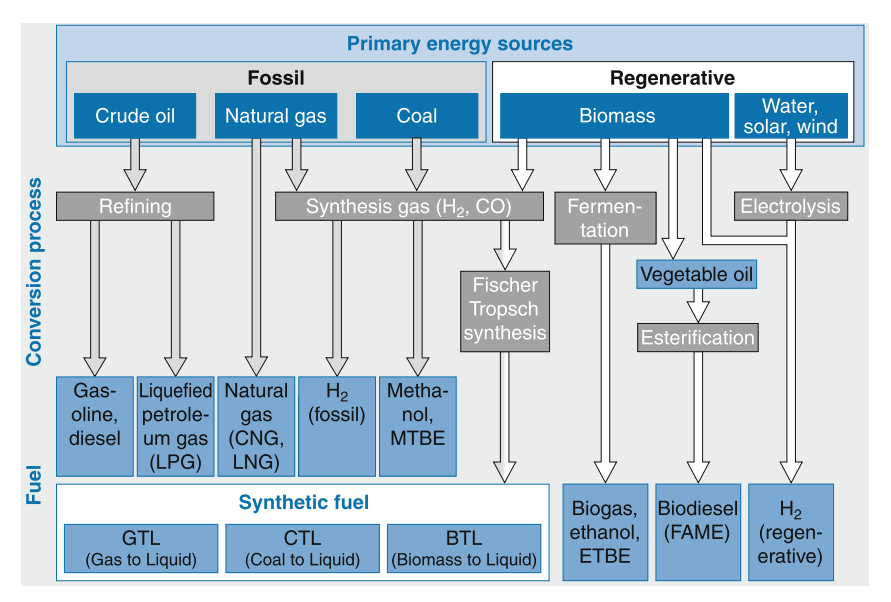
\includegraphics[width=0.95\textwidth]{img/energy.png}
  \caption{Primary Energy Sources.}
  \label{fig:Primary Energy Sources }
\end{figure}

\subsubsection*{Compression Ratio}
Compression ratio is a fundamental parameter used to describe the internal combustion process in an engine. It represents the ratio of the total cylinder volume when the piston is at the bottom of its stroke (bottom dead center) to the volume when the piston is at the top of its stroke (top dead center). In simpler terms, it quantifies how much the air-fuel mixture is compressed in the engine cylinder.\\

The compression ratio affects engine performance and efficiency in several ways, including its relationship with knocking:
\begin{itemize}
  \item Engine Power: A higher compression ratio generally leads to increased engine power output. This is because a greater compression ratio allows for more efficient combustion, resulting in better utilization of the fuel's energy.
  \item Engine Efficiency: A higher compression ratio can improve engine efficiency by extracting more energy from the fuel-air mixture. This is achieved through increased thermal efficiency, where more of the heat energy released during combustion is converted into useful work.
  \item Knocking: Knocking, also known as detonation, is an undesirable phenomenon where the air-fuel mixture in the cylinder detonates spontaneously before the spark plug ignites it. Knocking causes a knocking sound and can lead to engine damage if it occurs excessively.

\end{itemize}

The compression ratio has a significant impact on the likelihood of knocking. A higher compression ratio increases the cylinder pressure and temperature during compression, making the air-fuel mixture more prone to auto-ignition. If the fuel's octane rating is not high enough to resist knocking under the increased pressure and temperature, knocking can occur. The more compression ratio, the more knocking will happen.

To mitigate knocking, it is essential to use fuels with higher octane numbers in engines with higher compression ratios. Fuels with higher octane ratings have increased resistance to knocking, allowing them to withstand the higher pressures and temperatures associated with higher compression ratios.

\subsubsection*{H//C ratio}
The hydrogen-to-carbon ratio (H/C ratio) is a measure of the relative abundance of hydrogen and carbon atoms in a fuel molecule. It is commonly used to characterize the composition and properties of various fuels. The H/C ratio affects the energy content, combustion efficiency, and emission characteristics of a fuel.

\begin{figure}
  \centering
  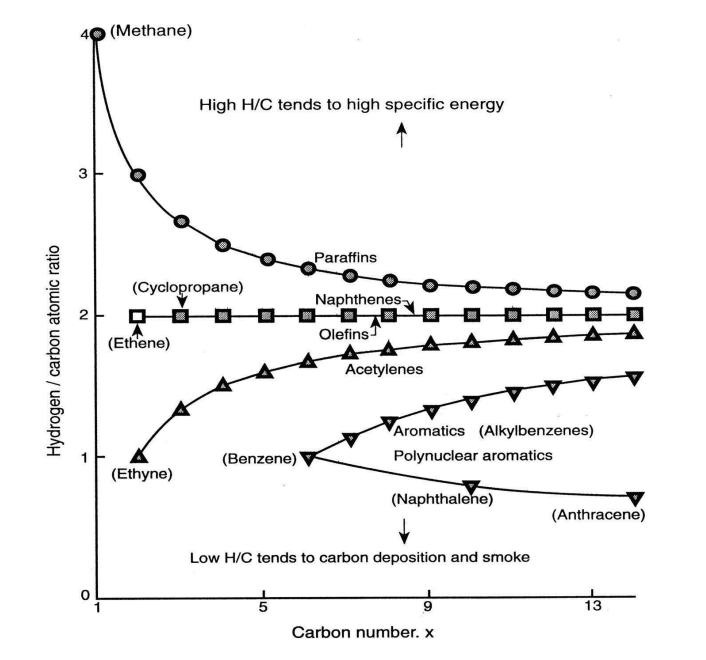
\includegraphics[width=0.75\textwidth]{img/hc_ratio.png}
  \caption{H:C atomic ratio of various inorganic hydrocarbon compounds.}
  \label{fig:Different H/C ratio }
\end{figure}

In general, fuels with higher H/C ratios tend to have higher energy content, as hydrogen has a higher energy content per unit mass compared to carbon. Fuels with higher H/C ratios also tend to burn more cleanly, producing fewer carbon dioxide (CO2) emissions and less particulate matter during combustion.


\subsubsection*{Diesel Fuel Specifications}
The terms 1-D, 2-D, and 4-D are commonly used to classify different grades or types of diesel fuel. These classifications are based on the volatility and viscosity characteristics of the fuel, and they are often associated with specific applications. Here's an overview of each type and their uses:

\begin{itemize}
  \item 1-D Diesel Fuel:
    \begin{itemize}
      \item 1-D diesel fuel is a lighter grade of diesel fuel that has a lower viscosity and higher volatility compared to 2-D and 4-D fuels.
      \item It is commonly used in colder climates or during winter months, as it has better cold flow properties and can prevent wax crystal formation at lower temperatures.
      \item 1-D fuel is often referred to as "winter diesel" or "arctic diesel" and is designed to perform well in low-temperature conditions.
      \item It is commonly used in applications such as transportation, agriculture, construction, and mining equipment operating in cold regions.
    \end{itemize}
  \item 2-D Diesel Fuel:
      \begin{itemize}
        \item 2-D diesel fuel is a mid-range grade of diesel fuel that has a moderate viscosity and volatility.
        \item It is suitable for use in a wide range of diesel engines and is the most commonly available type of diesel fuel in most areas.
        \item 2-D fuel is used in various applications, including passenger vehicles, trucks, buses, generators, boats, and industrial machinery.
        \item It is also used in heating systems, as it can be burned in oil furnaces or boilers for space heating.
      \end{itemize}

  \item 4-D Diesel Fuel:
      \begin{itemize}
        \item 4-D diesel fuel is a heavier grade of diesel fuel with a higher viscosity and lower volatility compared to 1-D and 2-D fuels.
        \item It is primarily used in industrial applications and heavy-duty engines that require more robust fuel properties.
        \item 4-D fuel is commonly used in large marine engines, locomotives, power generation, and industrial equipment.
        \item It may also be used in off-road vehicles and machinery, such as construction equipment and agricultural machinery.
      \end{itemize}

\end{itemize}

\subsubsection*{Automotive Fuels}
Automotive fuels are the types of fuels used to power vehicles, specifically designed for use in internal combustion engines found in cars, motorcycles, trucks, and other vehicles. The two primary types of automotive fuels are gasoline and diesel fuel.

\textbf{Gasoline}: Gasoline, also known as petrol, is a volatile fuel primarily used in spark-ignition engines. It is a mixture of hydrocarbons derived from crude oil through refining processes. Gasoline is designed to combust in spark-ignition engines, where a spark from the spark plug ignites the fuel-air mixture, generating power.

\textbf{Diesel Fuel}: Diesel fuel is a heavier and less volatile fuel used in compression-ignition engines, commonly known as diesel engines. It contains higher energy content compared to gasoline and is ignited through compression rather than a spark. Diesel engines compress the air in the cylinder, raising its temperature and allowing diesel fuel to ignite spontaneously upon injection into the cylinder.

Both gasoline and diesel fuel are refined from crude oil, but they have different properties and combustion characteristics due to variations in refining processes. These fuels are distributed through fuel stations or gas stations, where vehicles can be refueled.

Alternative automotive fuels, such as ethanol, biodiesel, natural gas (CNG/LNG), hydrogen, and electric power, are also gaining prominence as alternatives to traditional gasoline and diesel fuels. These alternative fuels aim to reduce emissions, enhance fuel efficiency, and promote environmental sustainability in the transportation sector.

\subsubsection*{Typical Properties of Automotive fuels}
\textbf{Gasoline}:
  \begin{itemize}
    \item Octane Number: Measures the fuel's resistance to knocking or premature combustion.
    \item Vapor Pressure: Indicates the fuel's ability to vaporize at specific temperatures.
    \item Reid Vapor Pressure (RVP): Measures the vapor pressure of gasoline at 100 degrees Fahrenheit (37.8 degrees Celsius).
    \item Ethanol Content: Percentage of ethanol added as an oxygenate in gasoline.
    \item Energy Content: Amount of energy per unit volume (megajoules per liter or British thermal units per gallon).
    \item Density: Mass per unit volume of gasoline.
    \item Research Octane Number (RON): A measure of gasoline's resistance to knocking under controlled conditions.
    \item Motor Octane Number (MON): A measure of gasoline's resistance to knocking under more severe conditions.
  \end{itemize}

\textbf{Diesel Fuel}:
    \begin{itemize}
      \item Cetane Number: Measures the ignition quality of diesel fuel.
      \item Sulfur Content: Amount of sulfur present in diesel fuel, which affects emissions.
      \item Energy Content: Amount of energy per unit volume (megajoules per liter or British thermal units per gallon).
      \item Density: Mass per unit volume of diesel fuel.
      \item Lubricity: Ability of diesel fuel to provide lubrication to fuel system components.
      \item Distillation Range: The temperature range at which different components of diesel fuel vaporize.
      \item Cold Flow Properties: Parameters such as the cloud point, pour point, and cold filter plugging point (CFPP) that determine the fuel's performance in cold temperatures.
    \end{itemize}


  \subsubsection*{Aviation Fuels}
  Aviation fuel, also known as aviation gasoline (Avgas) and jet fuel, is a specialized type of fuel designed for use in aircraft. The properties of aviation fuel are specifically formulated to meet the unique requirements of aviation engines. \textbf{Typically aviation fuels are similar to Kerosine, but sulfer content very low.}

  Here's an overview of aviation fuel and its typical properties:

\textbf{Aviation Gasoline (Avgas)}:

\begin{itemize}
  \item Aviation gasoline is primarily used in piston-engine aircraft.
  \item Octane Rating: Avgas has high octane ratings, typically ranging from 91 to 130, to prevent knocking in high-performance aircraft engines.
  \item Lead Content: Some Avgas formulations may contain lead additives for added octane rating. However, there is a global push to transition to unleaded Avgas to minimize environmental impact.
  \item Density: Avgas has a specific gravity that varies depending on the specific formulation but typically falls between 0.72 and 0.78 kg/L (6.0 to 6.5 lb/gal).
  \item Vapor Pressure: Avgas has controlled vapor pressure to ensure reliable fuel delivery in aircraft systems across a range of altitudes and temperatures.
  \item Flash Point: The flash point of Avgas is typically around -40 to -45 degrees Celsius (-40 to -49 degrees Fahrenheit), indicating its low flammability.
\end{itemize}


\textbf{Jet Fuel}:
\begin{itemize}
  \item Jet fuel is used in gas turbine engines, including turbojets, turbofans, and turboprops.
  \item Jet A and Jet A-1: Jet A and Jet A-1 are the most common types of jet fuel used internationally. They have similar properties and are often interchangeable.
  \item Jet A/A-1 is a kerosene-based fuel with a relatively high flash point, making it less volatile than gasoline.
  \item Density: Jet fuel has a specific gravity around 0.8 kg/L (6.7 lb/gal).
  \item Energy Content: Jet fuel has a high energy content, typically around 35 to 42 megajoules per liter (130,000 to 160,000 British thermal units per gallon).
  \item Freezing Point: Jet fuel has a low freezing point to ensure it remains liquid at low temperatures encountered at high altitudes.
  \item Sulfur Content: International standards, such as Jet A-1, mandate low sulfur content (typically less than 0.3\% mass) to reduce emissions.
\end{itemize}



\newpage

\section{Lecture 3: Topic}
\subsection*{Date: DD/MM/YYYY}


\newpage

\section{Lecture 4: Equilibrium Composition (ISO-Octane at 30 bar)}
\hfill Date: 17/06/2023
\subsection*{Points}
\begin{enumerate}
  \item \textbf{Equivalence Ratio}: Equivalence ratio in an internal combustion engine refers to the ratio of the actual air-fuel mixture to the stoichiometric air-fuel ratio. It determines the richness or leanness of the mixture and affects combustion efficiency, power output, fuel consumption, and emissions. Operating at the stoichiometric ratio provides a balance between efficiency and emissions, but adjustments to the equivalence ratio can be made for optimal performance under different conditions. 
  \item Generally Equivalence ratio is maintained near 1. 
  \item At 500°C octane break down in other compounds like - Methane, Ethane, Butane or others. More than 100 radicals are produced. They further reacts and continue. 
  \item Bigger bond, like - (C-C) bond breaks and bond energy released and heat produced.
  \item H radicals are most critical. The fuel burning will increase in huge amount, if $H_2$ gas is added. 
  \item If fuel percentage is increased, they won't get enough time for fully burning. As a result incomplete burning will occur. Although there will be incomplete burning, there will produce a lot energy. Because of breaking bonds and energy releases. Increase in fuel will not good for the efficiency, but for power, it'll be good. 
  \item If fuel is higher, incomplete combustion will occur and $CO$ (carbon monoxide) like substance will be produced. 
  \item If everything remains same, the higher the RPM, the more power will be produced. 
  \item Fuel burning will be faster in presence of $H_2$ in air fuel mixure. 
  \item To get more power, $H_2$ gas is sucked to the cylinder from the exhaust gas. (As $H_2$ gas is there in exhaust gas) It's known as exhaust gas recirculation. 
  \item At 1750°C temperature, Produces gases in lean or rich condition are  totally different from eath other.
  \item Efficient engine (more than 50\%), their RPM are generally lower (nearly 100 RPM). As, In lower RPM, air fuel mixures will get enough time to burn fully.
  \item The less heat of combustion, the more less the specific heat capacity. 
  \item Maximum Flate temp at $\phi$ = 1.05. But for $\phi$ > 1, heat combustion and heat capacity will decay. 
\end{enumerate}

\vspace*{0.5cm}
\begin{center}
  \begin{tabular}{ccc}
    \hline
     & Air fuel ratio, $\left(\frac{A}{F}\right)_s$ & LHV \\
    \hline
   Methnol & 6.43 & 19.9 \\
    Octane & 15.03 & 44.4 \\
    \hline
  \end{tabular}
  \end{center}

  \subsubsection*{Which one is better: Methanol or Octane?}
  In spite of having more LHV in octane, it has a higher air-to-fuel ratio. That means, 1 portion of fuel will take 15.03 portion of air. As a result, it will occupy more volume in cylinder. On the otherhand, methanol has a lower LHV, also lower air-to-fuel ratio. But, for the same volume of cylinder, methanol will give better performance. As, more methanol can be contained inside the cylinder. \textbf{So, It can not be decided to choose a fuel, only observing the Heating values.}\\
  There are also some benefits of using alcohol as fuel. More compression ratio is better for IC engines. In normal car, knocking will be an issue when compression ratio is higher than 12. But, in case of alcohol, the compression ratio of 18 is enough good. That's why, sports car normally uses alcohol instead of octane for more power. The more the compression ratio, the more the efficiency. 
  
  \subsubsection*{Some Important Points}
  \begin{itemize}
    \item SIT (Self Ignition Temperature) of Diesel is lower than octane. So, diesel engine gives better performance as it needs less temperature to ignite. 
    \item The SIT of methane is high. That's why for ignition in CNG cars, it requires more temperature in spark plug and thus it becomes out of work. 
  \end{itemize}

  \subsubsection*{Combustion efficiency in ICEs}
  $$\eta_c = \frac{H_R (T_o) - H_P (T_o)}{m_f Q_{HV}}$$

  Efficiency will never be 100\%. Because, fuel attached with cylinder wall have less temperature, like - 300-400°C. Whereas, burn temperature in 2500°C. So, Fuel along with wall doesn't burn at ease and requires much time to burn out. \\

  Any fuel can be used in Fuel engine. But, in petrol engine, fuel needs to make vapor first, that's why efficiency is an issue here. 

  \vspace*{0.5cm}
  \section{Lecture 5: Combustion \& Flame}
  \hfill Date: 20/06/2023 \\

  For combustion three parameters are important: \textbf{Power, Efficiency \& Emission}\\


  \textbullet Flame: A rapid exothermic chemical reaction. \\
  \textbullet Flame:  Conventional spark-ignition (SI) flame is premixed unsteady turbulent flame, and the fuel-air mixture through which it propagates is in the
  gaseous state.

  Conventional spark-ignition (SI) flame is premixed unsteady turbulent
  flame, and the fuel-air mixture through which it propagates is in the
  gaseous state.

  Diesel engine (CI) combustion process is predominantly an unsteady
  turbulent diffusion flame, and the fuel is initially in the liquid phase\\

  \textbf{Premixed Flame}: fuel and oxidizer are essentially uniformly mixed
  prior to combustion. It is a rapid, essentially isobaric, exothermic
  reaction of gaseous fuel and oxidizer, and flame propagates as a thin
  zone with speeds of less than a few m/s.\\

  \textbf{Diffusion Flame}: reactants are not premixed and must mix together
  in the same region where reactions take place. It is dominated by the
  mixing of reactants, which can be either laminar or turbulent, and
  reaction takes place at the interface between the fuel and oxidizer

  \subsection*{Auto Ignition \& Self-Ignition Temperature:}
  \textbf{Auto Ignition Temperature:} The auto ignition temperature is the lowest temperature at which the air-fuel mixture can auto-ignite under specific conditions of pressure and composition. It is typically associated with gasoline engines and is the temperature at which knocking or detonation can occur if it is reached before the spark plug fires. The auto ignition temperature of gasoline is typically around 495-535 degrees Celsius (923-995 degrees Fahrenheit).

\textbf{Self Ignition Temperature:} The self-ignition temperature, also known as the ignition point or the ignition temperature, is the minimum temperature at which a fuel will self-ignite without the presence of an external ignition source. It is more commonly associated with diesel engines, where the fuel is injected into the hot, compressed air in the combustion chamber. The self-ignition temperature of diesel fuel is generally higher than that of gasoline, ranging from about 210-260 degrees Celsius (410-500 degrees Fahrenheit).

\subsubsection*{Effect of SIT \& AIT}
In general, for internal combustion engines, both gasoline and diesel, higher auto-ignition and self-ignition temperatures are preferred.\\

For auto-ignition in gasoline engines, a higher temperature threshold is preferred to prevent premature or uncontrolled combustion, such as knocking or detonation. Knocking can lead to engine damage, reduced performance, and increased emissions. Fuels with higher resistance to auto-ignition, indicated by higher auto-ignition temperatures, are desired to ensure proper combustion control and avoid these issues.\\

Similarly, in diesel engines, a higher self-ignition temperature is preferred. Diesel engines rely on the self-ignition of the fuel when injected into the compressed air. A higher self-ignition temperature ensures that ignition occurs at the intended timing and allows for efficient combustion. It also helps in avoiding spontaneous ignition during the compression stroke before the fuel injection, which can cause damage to the engine.\\

As the ignition temperature increases, the ignition time becomes faster and the ignition delay becomes shorter. Higher temperatures promote more efficient combustion by facilitating quicker and more complete fuel combustion. This, in turn, reduces the time it takes for the air-fuel mixture to ignite and lowers the delay between the ignition event and the start of combustion. However, it's important to note that the relationship between ignition temperature and ignition time can be influenced by various factors, including fuel properties, engine design, and operating conditions. 

\subsubsection*{Ignition delay (ID) depends on which factor:}
Factors influencing ignition delay in internal combustion engines include fuel properties (such as cetane number or octane rating),initial temperature, Density, turbulence swirl, compression ratio, air-fuel mixture composition, presence of inert gas, engine operating conditions (speed, load, temperature, pressure), ignition system effectiveness, and combustion chamber design.\\  

\subsection*{Minimum Ignition Energy}


\begin{figure}[h]
	\centering
  
	\subfigure[Ignition Delay]{
	  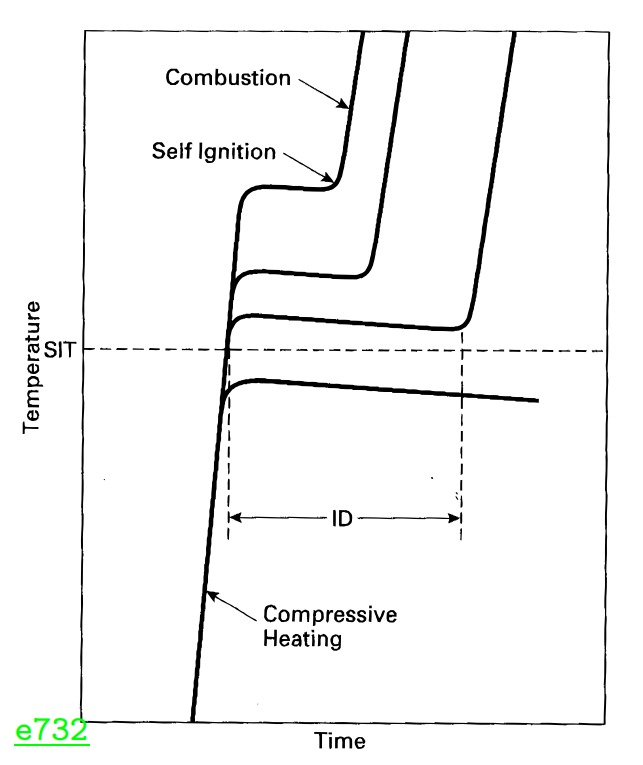
\includegraphics[width=0.45\linewidth]{img/ignition_delay.jpeg}
	  \label{fig:ID}
	}
	\hfill
	\subfigure[Critical Pressure vs critical temperature]{
	  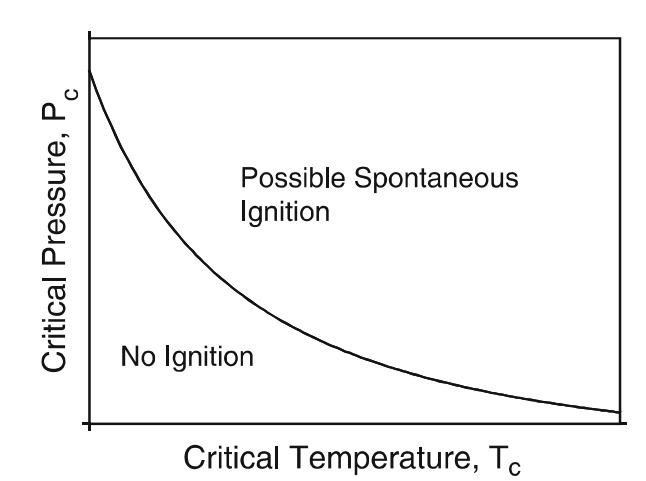
\includegraphics[width=0.45\linewidth]{img/critical_pv.jpeg}
	  \label{fig:const_vol}
	}
	
	\subfigure[electrode gap]{
	  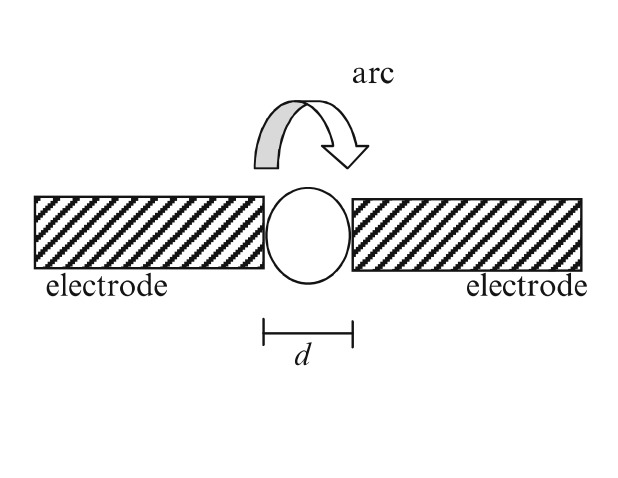
\includegraphics[width=0.45\linewidth]{img/min_egn_energy.jpeg}
	  \label{fig:const_pressure}
	}
	\hfill
	\subfigure[Minimum Ignition Energy]{
	  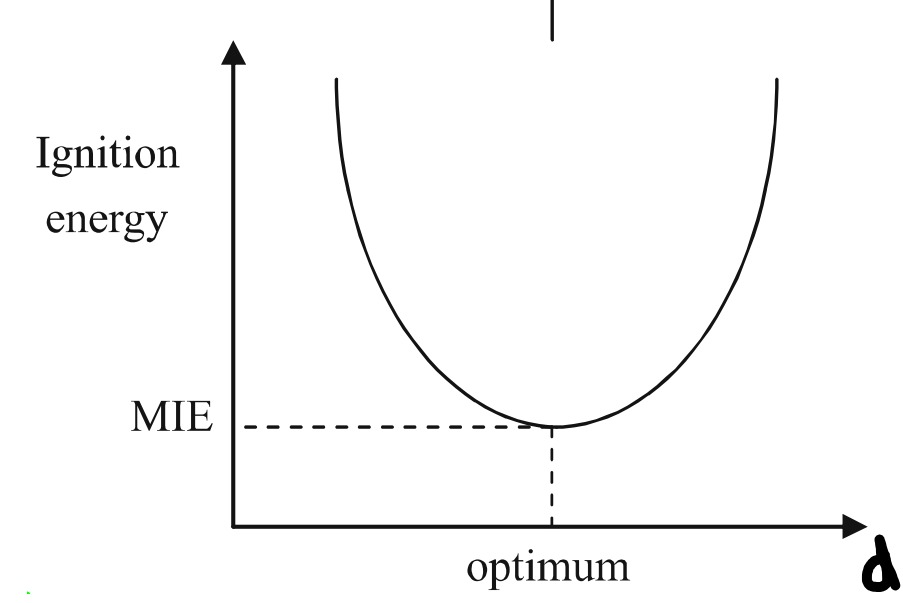
\includegraphics[width=0.45\linewidth]{img/min_egn_energy2.jpeg}
	  \label{fig:limited_const_vol_pre}
	}

	\label{fig:combustion_cycle}
  \end{figure}
  
  \begin{itemize}
    \item For lower d, heat loss to electrode is higher  (Heat loss $\propto \frac{1}{d}$)
    \item For higher d, volume increases ($d^3$) . The volume of air fuel mixure will be higher between the eletrodes. 
    \item so, Heat loss will be minimum at a particular distance d. (shown on the figure)
  \end{itemize}

  \subsection*{flammability limit}
  Flammability limits, also known as explosive limits or flammable limits, refer to the range of concentrations of a combustible substance in a mixture with air that can support combustion. These limits define the lower flammable limit (LFL) and upper flammable limit (UFL) of the substance.

\textbf{The lower flammable limit (LFL)} is the minimum concentration of the combustible substance in the air below which there is insufficient fuel for combustion to occur. At concentrations below the LFL, the mixture is too lean to sustain a flame or ignition.

\textbf{The upper flammable limit (UFL)} is the maximum concentration of the combustible substance in the air above which there is too much fuel for combustion to occur. At concentrations above the UFL, the mixture is too rich to sustain a flame or ignition.

Within the flammability limits, the mixture is within the range where combustion can occur if an ignition source is present. This range is often referred to as the flammable range.

The Lower Flammable Limit (LFL) and Upper Flammable Limit (UFL) can depend on temperature. Changes in temperature can affect the flammability limits of a substance. In general, as the temperature increases, the flammability limits tend to widen.

Flame speed significantly increase by turbulance. 

\subsubsection*{How Flame works:}
Nearest molecule of flame reaches the SIT, then burn and increase the furthur temperature of next molecules and propagate to the forwards. 

\begin{figure}[h]
  \begin{center}
    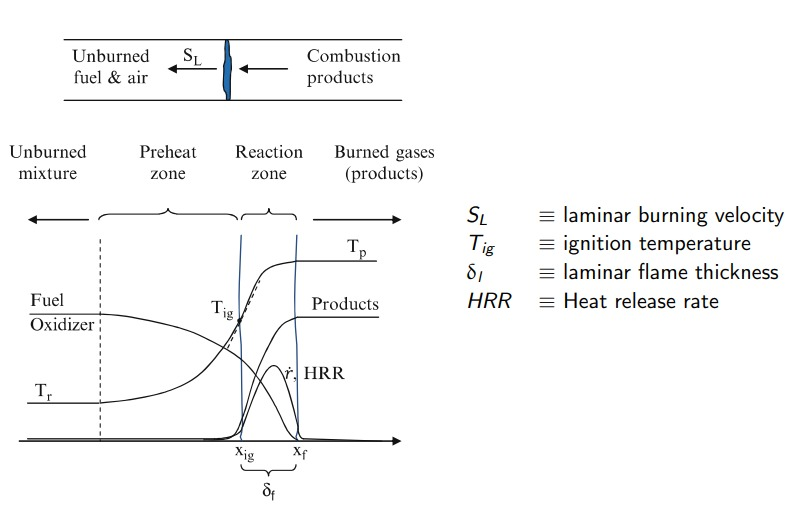
\includegraphics[width=0.95\linewidth]{img/flame_graph.jpeg}
  \end{center}
\end{figure}

\end{document}
